% !TEX TS-program = lualatex
% !TEX encoding = UTF-8 Unicode
\documentclass[12pt,a4paper]{article}

\IfFileExists{src/libs/body.tex}{% --- body.tex ---
\usepackage{pdfpages}
\usepackage{fontspec}
% Prefer Times New Roman when available; fall back in container environments.
\IfFontExistsTF{Times New Roman}{
  \setmainfont{Times New Roman}
}{
  \setmainfont{Liberation Serif}
}
\usepackage[vietnamese]{babel}

% Page layout and spacing
\usepackage[left=3cm,right=2cm,top=2cm,bottom=2cm]{geometry}
\usepackage{titlesec}
\usepackage{setspace}

% Silence noisy warnings
\usepackage{silence}
\WarningFilter{transparent}{Loading aborted}
\WarningFilter{hyperref}{The anchor of a bookmark and its parent's}

% Core packages
\usepackage{float}
\usepackage{svg}
\usepackage{graphicx}
\graphicspath{{assets/}{../assets/}{../../assets/}}
\svgpath{{assets/}{../assets/}{../../assets/}}
\usepackage{enumitem}
\usepackage{array}
\usepackage{tabularx}
\usepackage{multirow}
\usepackage[table]{xcolor}
\usepackage{ulem}
\usepackage{xurl}

% ====== THÊM 2 GÓI NÀY ĐỂ FIX LỖI ADJUSTBOX VÀ FOREST ======
\usepackage{adjustbox}
\usepackage[edges]{forest}
% ============================================================

% TikZ
\usepackage{tikz}

% ====== BỔ SUNG FIT, BACKGROUNDS, TREES VÀO DANH SÁCH ======
\usetikzlibrary{calc, arrows.meta, shapes.geometric, positioning, fit, backgrounds, trees}

% Table tuning
\renewcommand{\tabularxcolumn}[1]{m{#1}}
\hbadness=10000
\hfuzz=10000pt

% Shared commands
\newcommand{\subsecheading}[1]{%
    \par\vspace{2pt}%
    \hspace{1.5em}\textbf{#1}%
    \par\vspace{2pt}%
}
\newcommand{\introtext}[1]{%
    \par\hspace{3.0em}#1\par%
}
\newcommand{\StandaloneDocumentSetup}[2]{%
  \pagenumbering{arabic}%
  \ApplyStandardFooter{#1}{#2}%
}
\newcommand{\StandaloneSectionSetup}[2]{%
  \ApplyStandardFooter{#1}{#2}%
}

% Math
\usepackage{amsmath}

% Hyperref
\usepackage{hyperref}
\hypersetup{
    colorlinks=true,
    linkcolor=black,
    filecolor=magenta,
    urlcolor=blue,
}}{%
  \IfFileExists{../libs/body.tex}{% --- body.tex ---
\usepackage{pdfpages}
\usepackage{fontspec}
% Prefer Times New Roman when available; fall back in container environments.
\IfFontExistsTF{Times New Roman}{
  \setmainfont{Times New Roman}
}{
  \setmainfont{Liberation Serif}
}
\usepackage[vietnamese]{babel}

% Page layout and spacing
\usepackage[left=3cm,right=2cm,top=2cm,bottom=2cm]{geometry}
\usepackage{titlesec}
\usepackage{setspace}

% Silence noisy warnings
\usepackage{silence}
\WarningFilter{transparent}{Loading aborted}
\WarningFilter{hyperref}{The anchor of a bookmark and its parent's}

% Core packages
\usepackage{float}
\usepackage{svg}
\usepackage{graphicx}
\graphicspath{{assets/}{../assets/}{../../assets/}}
\svgpath{{assets/}{../assets/}{../../assets/}}
\usepackage{enumitem}
\usepackage{array}
\usepackage{tabularx}
\usepackage{multirow}
\usepackage[table]{xcolor}
\usepackage{ulem}
\usepackage{xurl}

% ====== THÊM 2 GÓI NÀY ĐỂ FIX LỖI ADJUSTBOX VÀ FOREST ======
\usepackage{adjustbox}
\usepackage[edges]{forest}
% ============================================================

% TikZ
\usepackage{tikz}

% ====== BỔ SUNG FIT, BACKGROUNDS, TREES VÀO DANH SÁCH ======
\usetikzlibrary{calc, arrows.meta, shapes.geometric, positioning, fit, backgrounds, trees}

% Table tuning
\renewcommand{\tabularxcolumn}[1]{m{#1}}
\hbadness=10000
\hfuzz=10000pt

% Shared commands
\newcommand{\subsecheading}[1]{%
    \par\vspace{2pt}%
    \hspace{1.5em}\textbf{#1}%
    \par\vspace{2pt}%
}
\newcommand{\introtext}[1]{%
    \par\hspace{3.0em}#1\par%
}
\newcommand{\StandaloneDocumentSetup}[2]{%
  \pagenumbering{arabic}%
  \ApplyStandardFooter{#1}{#2}%
}
\newcommand{\StandaloneSectionSetup}[2]{%
  \ApplyStandardFooter{#1}{#2}%
}

% Math
\usepackage{amsmath}

% Hyperref
\usepackage{hyperref}
\hypersetup{
    colorlinks=true,
    linkcolor=black,
    filecolor=magenta,
    urlcolor=blue,
}}{% --- body.tex ---
\usepackage{pdfpages}
\usepackage{fontspec}
% Prefer Times New Roman when available; fall back in container environments.
\IfFontExistsTF{Times New Roman}{
  \setmainfont{Times New Roman}
}{
  \setmainfont{Liberation Serif}
}
\usepackage[vietnamese]{babel}

% Page layout and spacing
\usepackage[left=3cm,right=2cm,top=2cm,bottom=2cm]{geometry}
\usepackage{titlesec}
\usepackage{setspace}

% Silence noisy warnings
\usepackage{silence}
\WarningFilter{transparent}{Loading aborted}
\WarningFilter{hyperref}{The anchor of a bookmark and its parent's}

% Core packages
\usepackage{float}
\usepackage{svg}
\usepackage{graphicx}
\graphicspath{{assets/}{../assets/}{../../assets/}}
\svgpath{{assets/}{../assets/}{../../assets/}}
\usepackage{enumitem}
\usepackage{array}
\usepackage{tabularx}
\usepackage{multirow}
\usepackage[table]{xcolor}
\usepackage{ulem}
\usepackage{xurl}

% ====== THÊM 2 GÓI NÀY ĐỂ FIX LỖI ADJUSTBOX VÀ FOREST ======
\usepackage{adjustbox}
\usepackage[edges]{forest}
% ============================================================

% TikZ
\usepackage{tikz}

% ====== BỔ SUNG FIT, BACKGROUNDS, TREES VÀO DANH SÁCH ======
\usetikzlibrary{calc, arrows.meta, shapes.geometric, positioning, fit, backgrounds, trees}

% Table tuning
\renewcommand{\tabularxcolumn}[1]{m{#1}}
\hbadness=10000
\hfuzz=10000pt

% Shared commands
\newcommand{\subsecheading}[1]{%
    \par\vspace{2pt}%
    \hspace{1.5em}\textbf{#1}%
    \par\vspace{2pt}%
}
\newcommand{\introtext}[1]{%
    \par\hspace{3.0em}#1\par%
}
\newcommand{\StandaloneDocumentSetup}[2]{%
  \pagenumbering{arabic}%
  \ApplyStandardFooter{#1}{#2}%
}
\newcommand{\StandaloneSectionSetup}[2]{%
  \ApplyStandardFooter{#1}{#2}%
}

% Math
\usepackage{amsmath}

% Hyperref
\usepackage{hyperref}
\hypersetup{
    colorlinks=true,
    linkcolor=black,
    filecolor=magenta,
    urlcolor=blue,
}}%
}
\IfFileExists{src/libs/header.tex}{% --- header.tex ---
\usepackage{fancyhdr}
\setlength{\headheight}{15.5pt} % Thêm dòng này để fix cảnh báo chiều cao
%\setlength{\headheight}{14.5pt}
\addtolength{\topmargin}{-2.5pt}

\pagestyle{fancy}
\fancyhf{}
\renewcommand{\headrulewidth}{0pt}
\renewcommand{\footrulewidth}{0pt}

\newcommand{\ApplyStandardHeader}{%
  \fancyhead[L]{%
    \begin{minipage}[t]{0.795\linewidth}%
      UIT \textbar{} SS004.F21 \textbar{} Nhóm 03 \textbar{} Đồ án cuối kỳ%
    \end{minipage}%
    \vrule%
    \begin{minipage}[t]{0.185\linewidth}%
      \centering cTetris%
    \end{minipage}%
  }%
}

\ApplyStandardHeader
}{%
  \IfFileExists{../libs/header.tex}{% --- header.tex ---
\usepackage{fancyhdr}
\setlength{\headheight}{15.5pt} % Thêm dòng này để fix cảnh báo chiều cao
%\setlength{\headheight}{14.5pt}
\addtolength{\topmargin}{-2.5pt}

\pagestyle{fancy}
\fancyhf{}
\renewcommand{\headrulewidth}{0pt}
\renewcommand{\footrulewidth}{0pt}

\newcommand{\ApplyStandardHeader}{%
  \fancyhead[L]{%
    \begin{minipage}[t]{0.795\linewidth}%
      UIT \textbar{} SS004.F21 \textbar{} Nhóm 03 \textbar{} Đồ án cuối kỳ%
    \end{minipage}%
    \vrule%
    \begin{minipage}[t]{0.185\linewidth}%
      \centering cTetris%
    \end{minipage}%
  }%
}

\ApplyStandardHeader
}{% --- header.tex ---
\usepackage{fancyhdr}
\setlength{\headheight}{15.5pt} % Thêm dòng này để fix cảnh báo chiều cao
%\setlength{\headheight}{14.5pt}
\addtolength{\topmargin}{-2.5pt}

\pagestyle{fancy}
\fancyhf{}
\renewcommand{\headrulewidth}{0pt}
\renewcommand{\footrulewidth}{0pt}

\newcommand{\ApplyStandardHeader}{%
  \fancyhead[L]{%
    \begin{minipage}[t]{0.795\linewidth}%
      UIT \textbar{} SS004.F21 \textbar{} Nhóm 03 \textbar{} Đồ án cuối kỳ%
    \end{minipage}%
    \vrule%
    \begin{minipage}[t]{0.185\linewidth}%
      \centering cTetris%
    \end{minipage}%
  }%
}

\ApplyStandardHeader
}%
}
\IfFileExists{src/libs/footer.tex}{% --- footer.tex ---
\usepackage{lastpage}

\newcommand{\ApplyStandardFooter}[2]{%
  \fancyfoot[L]{%
    \begin{minipage}[t]{0.795\linewidth}%
      Document ID: #1%
    \end{minipage}%
    \vrule%
    \begin{minipage}[t]{0.185\linewidth}%
      \centering\thepage/\pageref{#2}%
    \end{minipage}%
  }%
  \fancypagestyle{plain}{%
    \fancyhf{}%
    \renewcommand{\headrulewidth}{0pt}%
    \renewcommand{\footrulewidth}{0pt}%
    \ApplyStandardHeader%
    \fancyfoot[L]{%
      \begin{minipage}[t]{0.795\linewidth}%
        Document ID: #1%
      \end{minipage}%
      \vrule%
      \begin{minipage}[t]{0.185\linewidth}%
        \centering\thepage/\pageref{#2}%
      \end{minipage}%
    }%
  }%
  \pagestyle{fancy}%
}
}{%
  \IfFileExists{../libs/footer.tex}{% --- footer.tex ---
\usepackage{lastpage}

\newcommand{\ApplyStandardFooter}[2]{%
  \fancyfoot[L]{%
    \begin{minipage}[t]{0.795\linewidth}%
      Document ID: #1%
    \end{minipage}%
    \vrule%
    \begin{minipage}[t]{0.185\linewidth}%
      \centering\thepage/\pageref{#2}%
    \end{minipage}%
  }%
  \fancypagestyle{plain}{%
    \fancyhf{}%
    \renewcommand{\headrulewidth}{0pt}%
    \renewcommand{\footrulewidth}{0pt}%
    \ApplyStandardHeader%
    \fancyfoot[L]{%
      \begin{minipage}[t]{0.795\linewidth}%
        Document ID: #1%
      \end{minipage}%
      \vrule%
      \begin{minipage}[t]{0.185\linewidth}%
        \centering\thepage/\pageref{#2}%
      \end{minipage}%
    }%
  }%
  \pagestyle{fancy}%
}
}{% --- footer.tex ---
\usepackage{lastpage}

\newcommand{\ApplyStandardFooter}[2]{%
  \fancyfoot[L]{%
    \begin{minipage}[t]{0.795\linewidth}%
      Document ID: #1%
    \end{minipage}%
    \vrule%
    \begin{minipage}[t]{0.185\linewidth}%
      \centering\thepage/\pageref{#2}%
    \end{minipage}%
  }%
  \fancypagestyle{plain}{%
    \fancyhf{}%
    \renewcommand{\headrulewidth}{0pt}%
    \renewcommand{\footrulewidth}{0pt}%
    \ApplyStandardHeader%
    \fancyfoot[L]{%
      \begin{minipage}[t]{0.795\linewidth}%
        Document ID: #1%
      \end{minipage}%
      \vrule%
      \begin{minipage}[t]{0.185\linewidth}%
        \centering\thepage/\pageref{#2}%
      \end{minipage}%
    }%
  }%
  \pagestyle{fancy}%
}
}%
}
\usepackage{docmute}

\hypersetup{pdftitle={Hướng dẫn sử dụng - Tổng hợp hệ thống}}

\begin{document}
\providecommand{\StandaloneSectionSetup}[2]{\ApplyStandardFooter{#1}{#2}}
\StandaloneSectionSetup{04-gameGuide}{LastPageUserGuide}
\onehalfspacing

\section{Hướng dẫn Sử dụng: Tổng hợp Hệ thống}

Tài liệu này hướng dẫn cách tương tác với ba phân hệ cốt lõi của trò chơi: \textbf{Phân hệ Cốt truyện}, \textbf{Phân hệ Bảng điều khiển}, và \textbf{Phân hệ Lõi trò chơi}.

% ======================================================================
% PHẦN 1: PHÂN HỆ CỐT TRUYỆN
% ======================================================================
\subsection{Phân hệ Cốt truyện (Màn hình Mở đầu \& Dẫn dắt)}

Đây là đoạn mở đầu ngắn 8 giây, đóng vai trò chào mừng và tải dữ liệu trước khi chuyển đến màn hình điều khiển chính.

\subsubsection{Giao diện Phiên bản 1 (Tự động hoàn toàn)}

\begin{figure}[htbp]
    \centering
    \begin{adjustbox}{max width=\linewidth}
    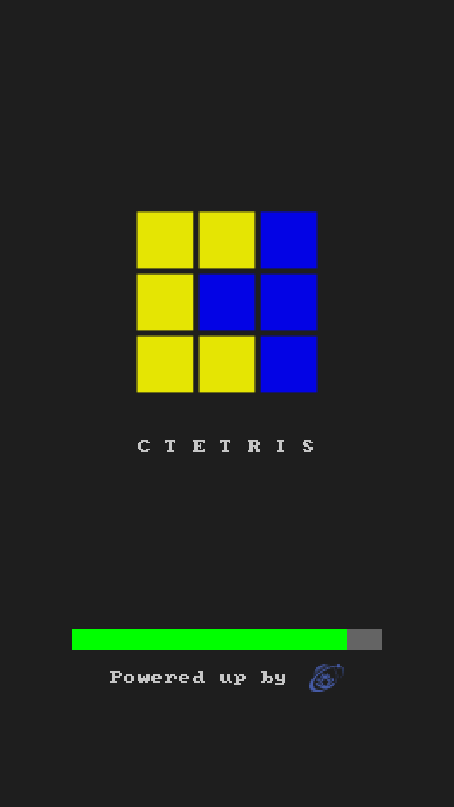
\includegraphics[width=0.3\textwidth]{08-gameStoryGuide-screenshot}
    \end{adjustbox}
    \\[10pt]
    \textit{\small Hình 8.1: Màn hình phân hệ Cốt truyện - Phiên bản 1}
\end{figure}

\begin{center}
\begin{adjustbox}{max width=\linewidth}
\begin{tabular}{|c|p{8cm}|}
    \hline
    \textbf{Thời điểm} & \textbf{Bạn sẽ thấy gì trên màn hình} \\
    \hline
    0 giây & Màn hình đen, các thành phần bắt đầu xuất hiện rất mờ. \\
    \hline
    2 giây & Biểu trưng và thông tin đã rõ khoảng 25\%, thanh tải dữ liệu lấp 1/4. \\
    \hline
    4 giây & Biểu trưng và thông tin hiện rõ 50\%, thanh tải đến giữa. \\
    \hline
    6 giây & Toàn bộ màn hình hiển thị rõ 75\%, thanh tải gần đầy. \\
    \hline
    8 giây & Mọi thành phần đạt độ rõ tối đa, thanh tải lấp đầy hoàn toàn. \\
    \hline
    > 8 giây & Tự động chuyển sang Phân hệ Bảng điều khiển (Trình đơn chính). \\
    \hline
\end{tabular}
\end{adjustbox}
\end{center}

\subsubsection{Giao diện Phiên bản 2 (Cốt truyện Tương tác)}

\begin{figure}[htbp]
    \centering
    \begin{adjustbox}{max width=\linewidth}
    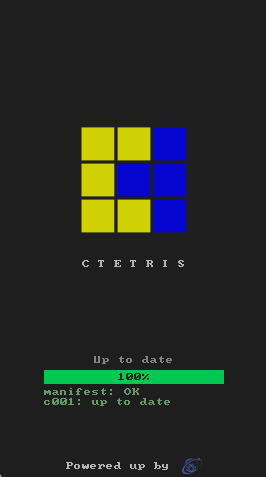
\includegraphics[width=0.3\textwidth]{08-gameStoryGuide-screenshot-v2}
    \end{adjustbox}
    \\[10pt]
    \textit{\small Hình 8.2: Màn hình phân hệ Cốt truyện - Phiên bản 2}
\end{figure}

\begin{center}
\begin{adjustbox}{max width=\linewidth}
    \includegraphics[page=1]{assets/tikz/diagrams-part4.pdf}
\end{adjustbox}
\end{center}

\textbf{Hai chế độ vận hành:}
\begin{center}
\begin{adjustbox}{max width=\linewidth}
    \includegraphics[page=2]{assets/tikz/diagrams-part4.pdf}
\end{adjustbox}
\end{center}

\subsubsection{Hệ thống Hội thoại}

\begin{figure}[htbp]
    \centering
    \begin{adjustbox}{max width=\linewidth}
    
\includegraphics[width=0.3\textwidth]{assets/08-gameStoryGuide-screenshot-v2-dialogue}
    \end{adjustbox}
    \\[10pt]
    \textit{\small Hình 8.3: Màn hình phân hệ Cốt truyện Phiên bản 2 - Hội thoại}
\end{figure}

\begin{center}
\begin{adjustbox}{max width=\linewidth}
    \includegraphics[page=3]{assets/tikz/diagrams-part4.pdf}
\end{adjustbox}
\end{center}

\subsubsection{Kiểm tra điều kiện sau 8 giây}
\begin{center}
\begin{adjustbox}{max width=\linewidth}
    \includegraphics[page=4]{assets/tikz/diagrams-part4.pdf}
\end{adjustbox}
\end{center}

% ======================================================================
% PHẦN 2: PHÂN HỆ BẢNG ĐIỀU KHIỂN
% ======================================================================
\subsection{Phân hệ Bảng điều khiển (Trung tâm Điều phối)}

Từ màn hình này bạn có thể bắt đầu ván đấu, xem kết quả, chọn câu chuyện, chỉnh cài đặt, và thoát ra.

\begin{center}
\begin{adjustbox}{max width=\linewidth}
    \includegraphics[page=5]{assets/tikz/diagrams-part4.pdf}
\end{adjustbox}
\end{center}

\subsubsection{Giao diện Phiên bản 1}
\begin{figure}[htbp]
    \centering
    \begin{adjustbox}{max width=\linewidth}
    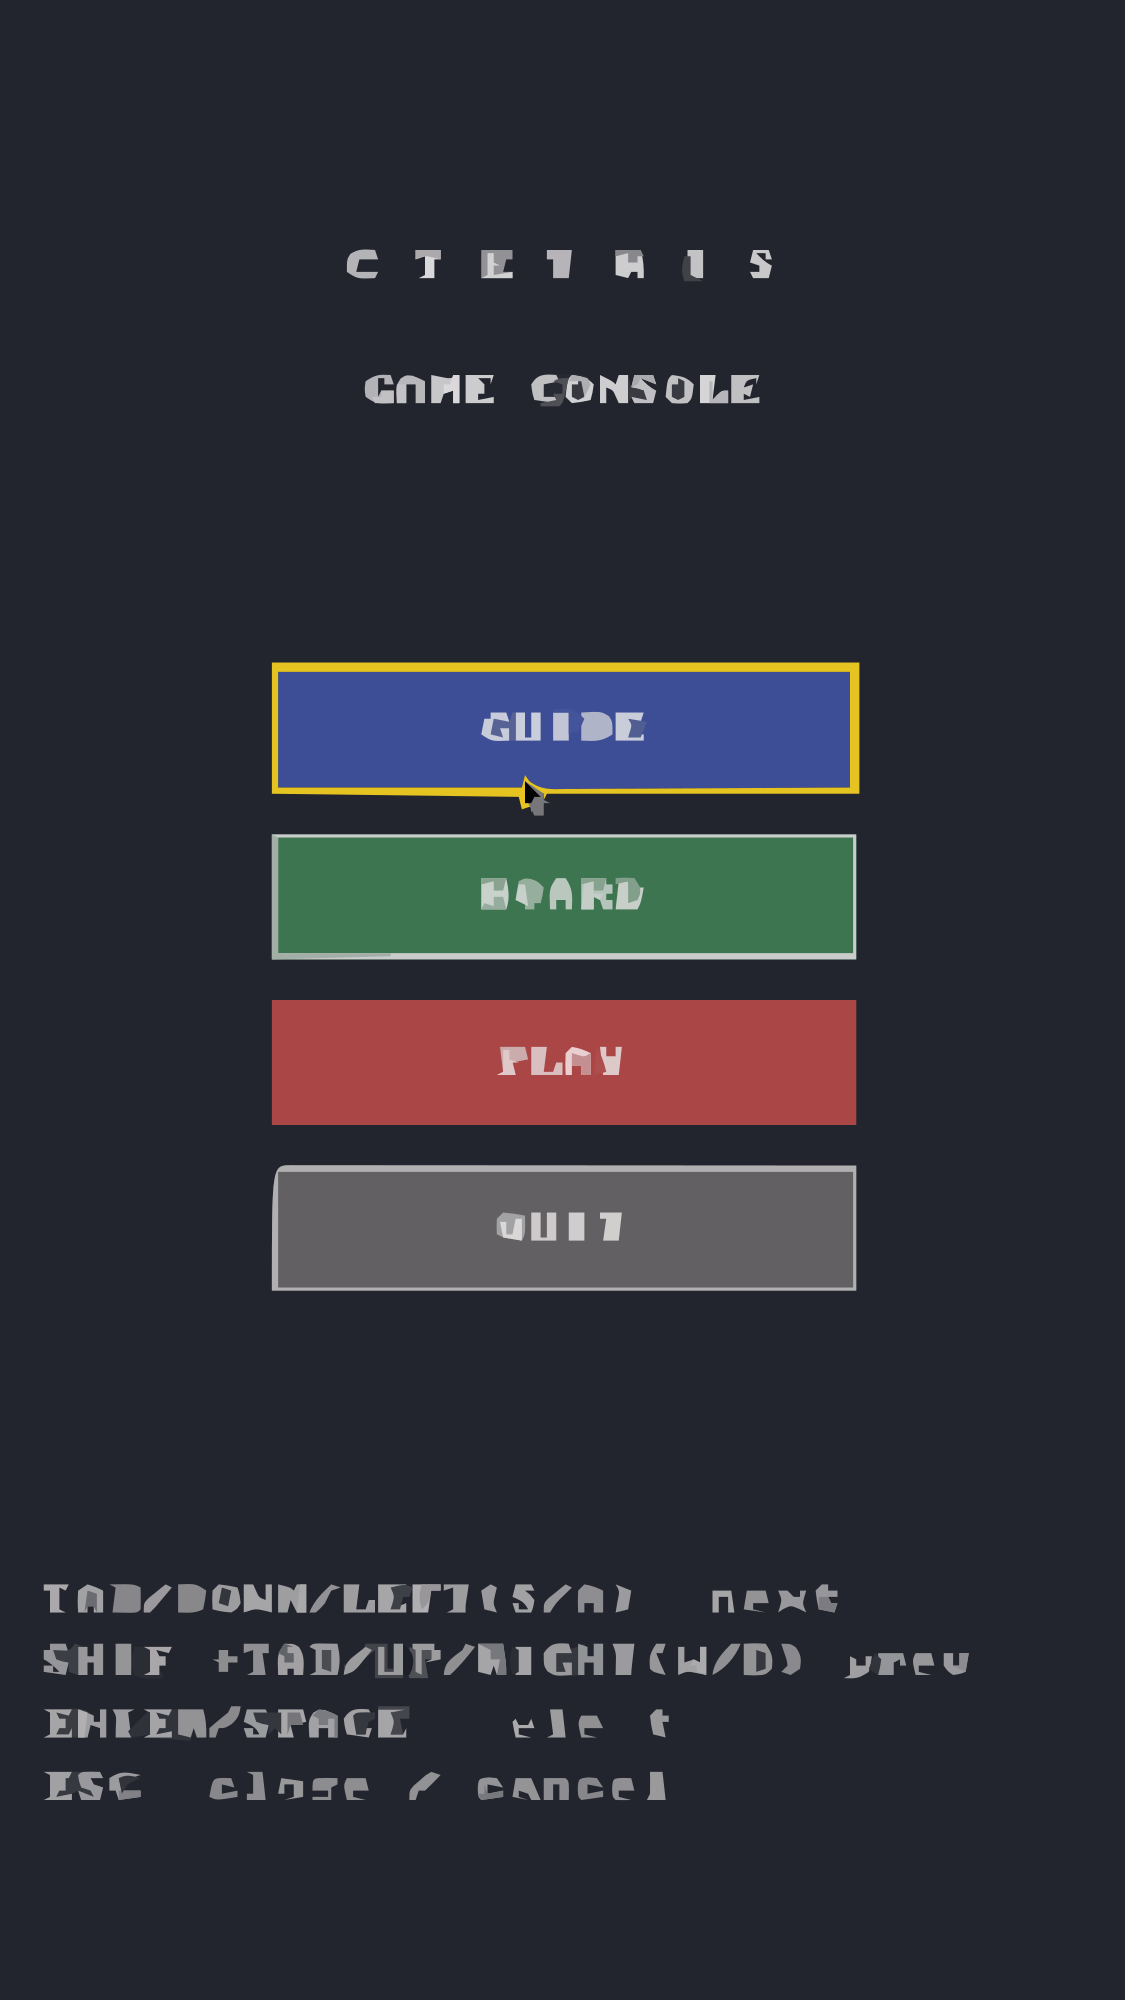
\includegraphics[width=0.3\textwidth]{09-gameConsoleGuide-screenshot}
    \end{adjustbox}
    \\[10pt]
    \textit{\small Hình 9.1: Màn hình phân hệ Bảng điều khiển - Phiên bản 1}
\end{figure}

\begin{center}
\begin{adjustbox}{max width=\linewidth}
\begin{tabular}{|l|l|p{6cm}|}
    \hline
    \textbf{Phím} & \textbf{Hành động} \\
    \hline
    \texttt{TAB} \,/\, \texttt{S} \,/\, \texttt{A} & Tiến tới nút kế tiếp. \\
    \hline
    \texttt{Shift+TAB} \,/\, \texttt{W} \,/\, \texttt{D} & Lùi về nút trước đó. \\
    \hline
    \texttt{ENTER} \,/\, \texttt{SPACE} & Chọn nút. \\
    \hline
    \texttt{ESC} & Nhảy về nút THOÁT. \\
    \hline
\end{tabular}
\end{adjustbox}
\end{center}

\subsubsection{Giao diện Phiên bản 2 (Thêm Cài đặt \& Cốt truyện)}
\begin{figure}[htbp]
    \centering
    \begin{adjustbox}{max width=\linewidth}
    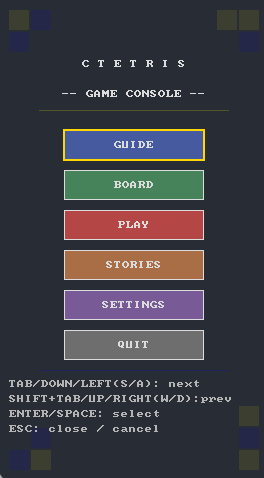
\includegraphics[width=0.3\textwidth]{09-gameConsoleGuide-screenshot-v2}
    \end{adjustbox}
    \\[10pt]
    \textit{\small Hình 9.2: Màn hình phân hệ Bảng điều khiển - Phiên bản 2}
\end{figure}

\begin{center}
\begin{adjustbox}{max width=\linewidth}
    \includegraphics[page=6]{assets/tikz/diagrams-part4.pdf}
\end{adjustbox}
\end{center}

\subsubsection{Các Cửa sổ Chức năng}
\begin{figure}[htbp]
    \centering
    \begin{minipage}[t]{0.24\textwidth}
        \vspace{0pt}
        \centering
        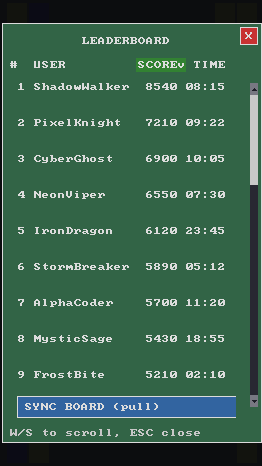
\includegraphics[width=\linewidth]{09-gameConsoleGuide-screenshot-v2-board}
        \vspace{5pt}
        \textit{\small Hình 9.3: Cửa sổ Xếp hạng}
    \end{minipage}\hfill
    \begin{minipage}[t]{0.24\textwidth}
        \vspace{0pt}
        \centering
        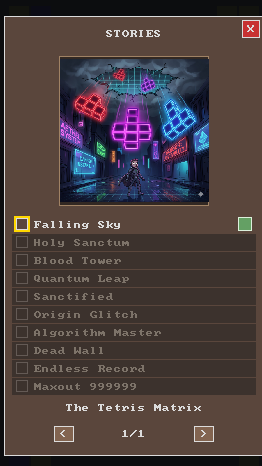
\includegraphics[width=\linewidth]{09-gameConsoleGuide-screenshot-v2-stories}
        \vspace{5pt}
        \textit{\small Hình 9.4: Cửa sổ Cốt truyện}
    \end{minipage}\hfill
    \begin{minipage}[t]{0.24\textwidth}
        \vspace{0pt}
        \centering
        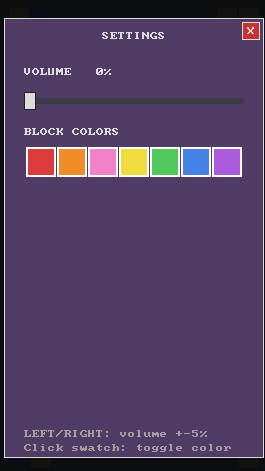
\includegraphics[width=\linewidth]{09-gameConsoleGuide-screenshot-v2-setting}
        \vspace{5pt}
        \textit{\small Hình 9.5: Cửa sổ Cài đặt}
    \end{minipage}\hfill
    \begin{minipage}[t]{0.24\textwidth}
        \vspace{0pt}
        \centering
        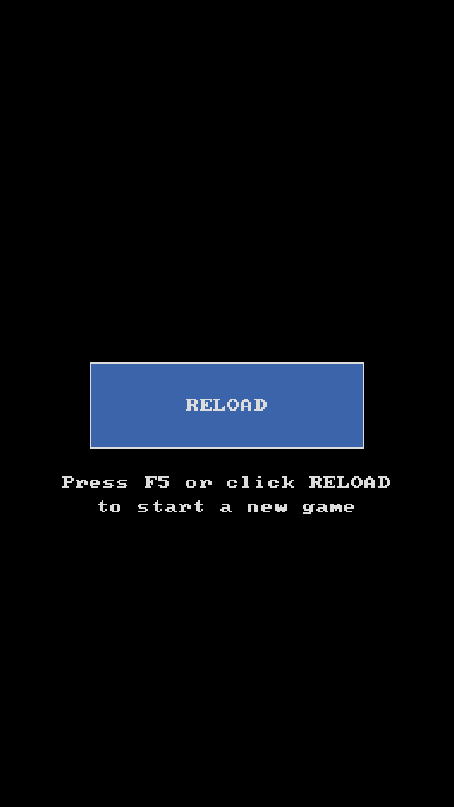
\includegraphics[width=\linewidth]{09-gameConsoleGuide-screenshot-v2-reload}
        \vspace{5pt}
        \textit{\small Hình 9.6: Cửa sổ Tải lại (Trình duyệt)}
    \end{minipage}
\end{figure}

\begin{center}
\begin{adjustbox}{max width=\linewidth}
\begin{tabular}{|l|p{8cm}|}
    \hline
    \textbf{Tính năng} & \textbf{Mô tả} \\
    \hline
    \textbf{Xếp hạng} & 4 chế độ sắp xếp: Điểm giảm/tăng dần, Thời gian mới/cũ nhất. \\
    \hline
    \textbf{Cốt truyện} & 3 trạng thái truyện: Đã khóa (mờ), Đã mở (chọn được), Đang chọn (chấm đậm). \\
    \hline
    \textbf{Cài đặt} & Chỉnh âm lượng (bằng phím Trái/Phải) và Bật/Tắt 7 màu khối. \\
    \hline
    \textbf{Tải lại} & Bấm F5 hoặc nút trên màn hình để khởi động lại trên nền Web. \\
    \hline
\end{tabular}
\end{adjustbox}
\end{center}

% ======================================================================
% PHẦN 3: PHÂN HỆ LÕI TRÒ CHƠI
% ======================================================================
\subsection{Phân hệ Lõi trò chơi (Game Engine)}

Đây là nơi bạn tận hưởng trải nghiệm xếp hình cốt lõi.

\subsubsection{Giao diện Phiên bản 1}
\begin{figure}[htbp]
    \centering
    \begin{adjustbox}{max width=\linewidth}
    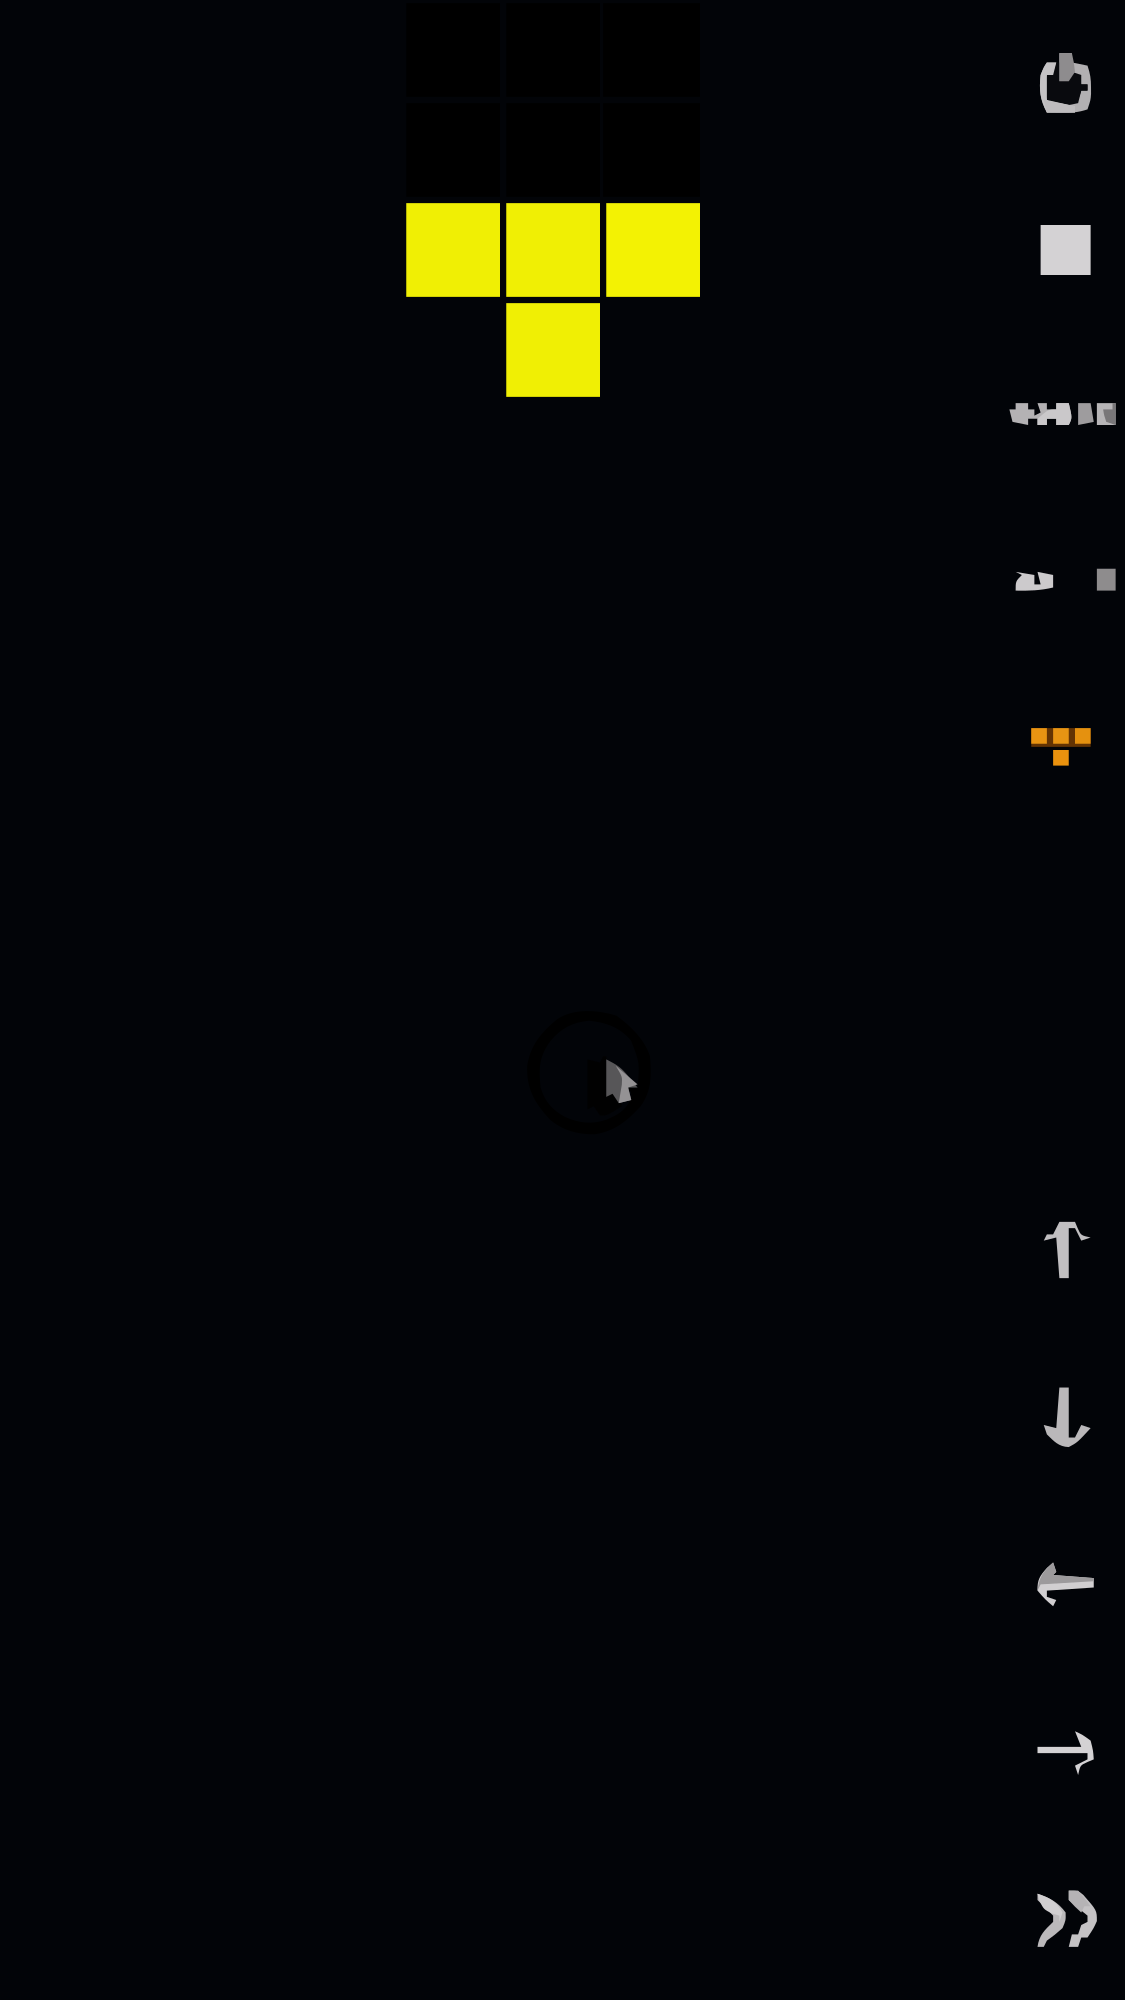
\includegraphics[width=0.3\textwidth]{10-gameCoreGuide-screenshot}
    \end{adjustbox}
    \\[10pt]
    \textit{\small Hình 10.1: Màn hình phân hệ Lõi trò chơi - Phiên bản 1}
\end{figure}

\begin{center}
\begin{adjustbox}{max width=\linewidth}
    \includegraphics[page=7]{assets/tikz/diagrams-part4.pdf}
\end{adjustbox}
\end{center}

\subsubsection{Giao diện Phiên bản 2}
\begin{figure}[htbp]
    \centering
    \begin{adjustbox}{max width=\linewidth}
    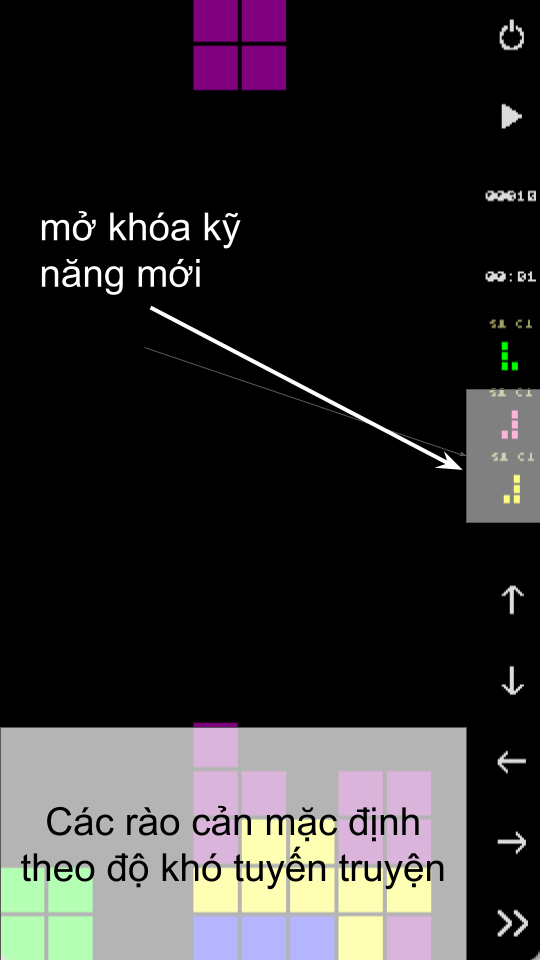
\includegraphics[width=0.3\textwidth]{10-gameCoreGuide-screenshot-v2}
    \end{adjustbox}
    \\[10pt]
    \textit{\small Hình 10.2: Màn hình phân hệ Lõi trò chơi - Phiên bản 2}
\end{figure}

\begin{center}
\begin{adjustbox}{max width=\linewidth}
    \includegraphics[page=8]{assets/tikz/diagrams-part4.pdf}
\end{adjustbox}
\end{center}

\begin{center}
\begin{adjustbox}{max width=\linewidth}
    \includegraphics[page=9]{assets/tikz/diagrams-part4.pdf}
\end{adjustbox}
\end{center}

\begin{center}
\begin{adjustbox}{max width=\linewidth}
    \includegraphics[page=10]{assets/tikz/diagrams-part4.pdf}
\end{adjustbox}
\end{center}

\subsubsection{Trạng thái Kết thúc}
\begin{figure}[htbp]
    \centering
    \begin{adjustbox}{max width=\linewidth}
    \includegraphics[width=0.3\textwidth]{10-gameCoreGuide-screenshot-V2-poweroff}
    \end{adjustbox}
    \\[10pt]
    \textit{\small Hình 10.3: Màn hình phân hệ Lõi trò chơi - Phiên bản 2 - Hộp thoại Tắt máy}
\end{figure}

\begin{center}
\begin{adjustbox}{max width=\linewidth}
\begin{tabular}{|l|p{8cm}|}
    \hline
    \textbf{Nút lệnh} & \textbf{Hành động} \\
    \hline
    \textbf{Khởi động lại} & Chơi ván mới ngay lập tức (Lưu CSDL). \\
    \hline
    \textbf{Bảng điều khiển} & Về Trình đơn chính (Lưu CSDL). \\
    \hline
    \textbf{Thoát} & Thoát game hoặc Tải lại trang (Lưu CSDL). \\
    \hline
    \textbf{Hủy} & Hủy Thoát (Chỉ dùng được nếu đang Tạm dừng). \\
    \hline
\end{tabular}
\end{adjustbox}
\end{center}

\label{LastPageUserGuide}
\end{document}